%%%%%%%%%%%%%%%%%%%%%%%%%%%%%%%%%%%%%
%% Master Thesis - Computer Engineering
%% Copyright 2009 Ricardo Alexandre Fiorelli, Erick Poletto
%% This document is distributed by the terms of the license
%% included in the file LICENCE.
%%%%%%%%%%%%%%%%%%%%%%%%%%%%%%%%%%%%%

%%%%%%%%%%%%%%%%%%%%%%%%%%%%%%%%%%%%%
%% Second Chapter
%% State of the Art
%%%%%%%%%%%%%%%%%%%%%%%%%%%%%%%%%%%%%

\chapter{State of the Art} \label{chap2:state_of_the_art}
    \section{Green ICT or Green Computing} \label{sec2:green_ict}
        Green ICT is the exploitation of a combination of techniques and approaches in ICT related resources in order to obtain more energy efficient use of computer related resources. In other words, Green ICT is a new term originated from ``Green Computing'', it is the research and development of projects, making use of Information and Communication Technology and related applications or softwares in order to monitor the energy spent by the computers, printers and all other computing equipment. Applying this approach, it is possible to make a responsible use of computers and related resources. It is a new paradigm that has the objective in the environment. In order to achieve this objective, it is necessary to understand and have the ability to analyze the information about the ICT components among workstations, servers, network, cooling and many others. The analysis of the information provided by the measures of the components is made through a set of tools, which will be explained in the chapter~\ref{chap3:methodology}. 
        
        The step by step to apply a green strategy is to analyze where in the data center is wasting more energy (``Assessment''), and only then act with correction and prevention interventions (``Action Plan''). For instance, when buying a new component, analyze how much energy it spends and opt for the ones that consumes less energy, also, use of thin clients as a substitute of the PC applications. Moreover, one has to re-analyze the data center and correct the energy wasting, considering more environmental friendly options such as virtualization, power management and proper habits. Regarding the energy consumption, it is a critical issue for IT organizations now a days, either the objective is the reduction of costs, environmental issues or keeping the data center running. In the United States alone, data centers consumed \$4.5 billion worth of electricity in 2006. Industry analyst Gartner~\cite{GartnetKumar07} estimates that over the next 5 years, most enterprise will spend as much energy as they spend on hardware infrastructure, power and air conditioning.
        
        Furthermore, It is also important to consider that there are some indirect objectives concerning green computing. Such objectives includes reduction of costs, reduction of carbon footprint and disposal of hazard elements to the environment. The reduction of costs is provided by the fact that if the energy consumed by the components is reduced, the payment in the electricity bill is directly reduced, also, when by applying the well management of the resources, the costs related to cooling, the space required for the data center and the efficiency of the computer components are all indirectly reduced. Probably, an study on the effect on ROI would show the benefits on cost.
    
        In the next section there is the explanation of all the approaches and categories for applying a green solution.
    
    \section{Computer Energy Management Categories} \label{sec2:energy_categories}

    In terms of hardware and equipment, the main measures to be taken towards a Green ICT environment can be grouped in the following categories:
    \begin{itemize}
        \item Workstation Configuration;
        \item Policies / Tools / Labels;
        \item Thin client architectures;
        \item Servers and Virtualization;
        \item Data Storage;
        \item Power Architectures;
        \item Data Center Infrastructure.
    \end{itemize}
    
    For each of those categories there are several types of information that are relevant to the evaluation of the current situation of power consumption. For each category there will be a corresponding description along with a number of possible interventions, either purely conceptual or available in the market.In some cases a numerical analysis will also be provided. This information will allow the creation of a methodology to identify critical consumption issues where an investment in green ICT would bring the greater savings.
    
    \subsection{Machine Configuration}\label{sec2:machine_configuration}
        This category represents the components used in a certain machine configuration. The component's performance and power consumption can be obtained from several sources, such as the manufacturer specifications, benchmarks and also direct measurements in the case of power consumption.
        The following are the dimensions that influence the final power consumption of a machine.
            \paragraph*{Single-core / Multi-core Processors} Processors in general affect the overall power consumption of the computer by means of the workload that is required by it. For example, if the computer is in idle (without any processes running) the energy consumed is less than if the computer stays in full workload, but the idle state does not mean anything to the efficiency, because it is needed a high workload (about 70\%) to have the best workload/power consumption ratio.
            %Tirei o cache pelo simples fato de que nao afeta na overall consumption
            %\paragraph*{Cache Memory} %TODO Type and dimension of 
            \paragraph*{RAM Memory} There are several types and dimensions of memories that should be analyzed, for instance the difference in operation in 2.5V in DDR SDRAM, when compared 3.3V in SDRAM significantly reduce the power consumption. When compating DDR and DDR2, The Table~\ref{tab:power_consumption_ram}\nocite{Cooke:2009:Online} compares the difference in power consumption of DDR and DDR2 under various circumstances and it shows that the power consumed by RAM, even on maximum workload (+4.5W), does not have much effect on the overall computer consumption (~220W).
\begin{table}[h!tb]
\centering \resizebox{\textwidth}{!}{ % Fazendo a tabela caber no espaco da pagina
\begin{tabular}{|c|c|c|c|c|c|c|}
\hline
\textbf{RAM Type } & \textbf{Size } & \textbf{Load } & \textbf{+12V1 } & \textbf{+5V } & \textbf{+3.3V } & \textbf{Rise from Baseline } \tnhl
\multicolumn{ 1}{|c|}{\textbf{PC3200 DDR }} & \multicolumn{ 1}{c|}{512 MB } & Idle  & 0.5A  & 0.6A  & 3.0A  & n/a  \tn \cline{ 3- 7}
\multicolumn{ 1}{|c|}{} & \multicolumn{ 1}{c|}{} & Memtest86  & No Change  & No Change  & +0.7A  & +2.3W  \tn \cline{ 2- 7}
\multicolumn{ 1}{|c|}{} & \multicolumn{ 1}{c|}{1 GB} & Idle  & No Change  & No Change  & +0.6A  & +2.0W  \tn \cline{ 3- 7}
\multicolumn{ 1}{|c|}{} & \multicolumn{ 1}{c|}{} & Memtest86  & No Change  & No Change  & +1.0A  & +3.3W  \tnhl
\multicolumn{ 1}{|c|}{\textbf{533 MHz DDR2 }} & \multicolumn{ 1}{c|}{512 MB } & Idle  & 0.5A  & 3.6A  & 0.5A  & n/a  \tn \cline{ 3- 7}
\multicolumn{ 1}{|c|}{} & \multicolumn{ 1}{c|}{} & Memtest86  & No Change  & +0.4A  & No Change  & +2.0W  \tn \cline{ 2- 7}
\multicolumn{ 1}{|c|}{} & \multicolumn{ 1}{c|}{1 GB} & Idle  & No Change  & No Change  & No Change  & No Change  \tn \cline{ 3- 7}
\multicolumn{ 1}{|c|}{} & \multicolumn{ 1}{c|}{} & Memtest86  & No Change  & +0.9A  & No Change  & +4.5W \tnhl
\end{tabular}}
\caption{Power Consumption: RAM}
\label{tab:power_consumption_ram}
\end{table}
            \paragraph*{Hard Drives and Mass Memory} Power consumption in this case is affected mainly by design of the hard drive's spindle motor and the number and size of the spindle platters and, also,other components such as the actuator and controller board. Also, solid-state and flash drives reduce significantly the power consumed by the component, Figure~\ref{fig:power_consumption_harddrive} shows this difference.%XXX melhorar essa parte
            \begin{figure}[h!tb]
                    \centering
                    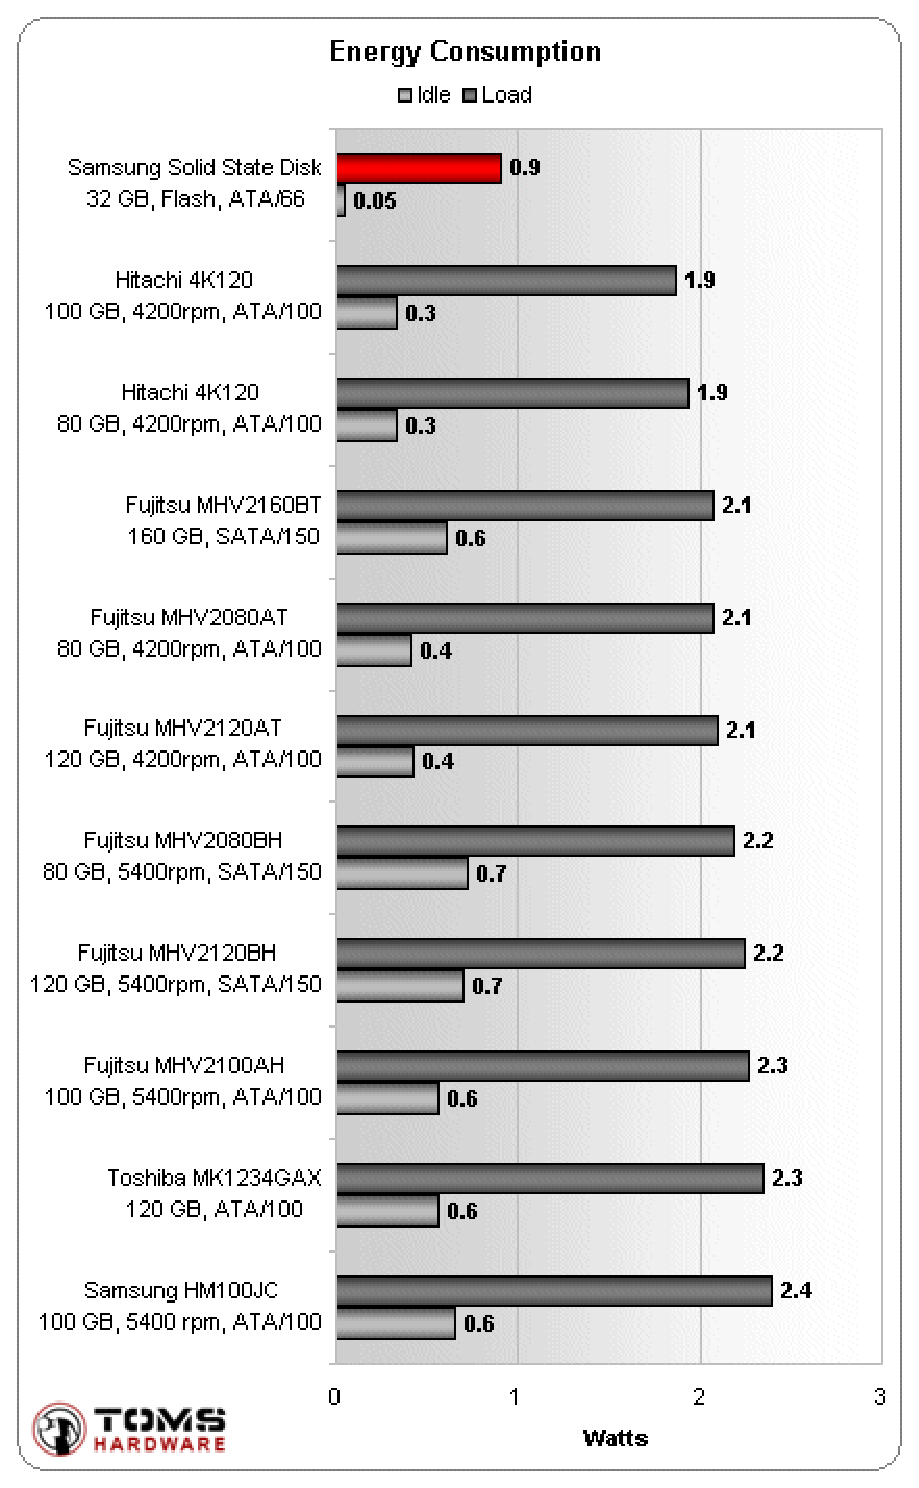
\includegraphics[scale=0.6]{graphics/power_consumption_harddrive}
                    \caption{Power Consumption for Hard-drives}
                    \label{fig:power_consumption_harddrive}
                \end{figure}
            \paragraph*{Chassis} Concerning power supply, fans or other PC components not belonging to the main parts, it is necessary to require quality other than price. Heating and cooling are really where the power consumption goes. Most computers only make up a fairly small percentage of your electrical bill. One should never underestimate the efficiency of the power supply, because most low quality ones are only about 45-55\% efficient, whereas it is possible to achieve more than 80\%.
            \paragraph*{Monitor Type} As shown by Table~\ref{tab:energy_used_monitor}\footnote{\url{http://michaelbluejay.com/electricity/computers.html}}, flat panel liquid crystal display (LCD) monitors power consumption equals to half the power of conventional CRT monitors. LCD monitors also dissipate less heat, which helps to reduce air conditioning costs. Another interesting point is that either LCD or CRT monitors consume the same amount of energy with or without screensavers. As LCD monitors do not consume much energy when turned off, that would be the best solution for idle computers.
\begin{table}[h!tb]
        \centering
        \begin{tabular}{|c|c|}
        \hline
        \multicolumn{ 2}{|c|}{{\bf Monitors}} \tnhl
        Typical 17" CRT &   80 watts \tnhl
        Typical 17" LCD &   35 watts \tnhl
        Apple MS 17" CRT$^a$ &   63 watts \tnhl
        Apple MS 17" CRT$^b$ &   54 watts \tnhl
        Screen saver$^c$ & same as above \tnhl
        Sleeping monitor$^d$ & 0-15 watts \tnhl
        Monitor turned off at switch & 0-10 watts \tnhl
        \end{tabular}  \linebreak
        $^a$ mostly white (blank IE window) \linebreak
        $^b$ mostly black (black Windows desktop with just a few icons)\linebreak
        $^c$ any image on screen\linebreak
        $^d$ dark screen
        \captionof{table}{Energy used by Monitors} 
\label{tab:energy_used_monitor}
    \end{table}

    \subsection{Policies / Tools / Labels} \label{sec2:policies_tools_labels}
        The amount of saved energy depends also on policies that regard technology acquisition and IT management, which may be enforced by a variety of specialized tools. Examples of policies that regard equipment acquisition are: the acquisition of new computers or components labeled as green by the manufacturer, purchase of computers with multi-core processors and even to discourage the purchase of specific kinds of hardware such as dual or large monitors and graphic cards. Another kind of policy relates to the management of the machines. One example of the latter is to turn off workstations or servers if they are going to be unused for a long time. This kind of measure is particularly efficient as a computer in idle mode uses 20 to 50 times the power of a computer in standby mode
\footnote{\url{http://www.cosn.org/Initiatives/GreenComputing/EnergyUse/tabid/4515/Default.aspx}}.
        
    \begin{table}[h!tb]
        \centering
        \begin{tabular}{|c|c|}
        \hline
        \multicolumn{ 2}{|c|}{{\bf Computers}} \tnhl
        Desktop Computer & 60-250 watts \tnhl
        On screen Saver$^a$ & 60-250 watts \tnhl
        Sleep / Standby & 1-6 watts \tnhl
        Laptop & 15-45 watts \tnhl
        \end{tabular}\linebreak
        $^a$ no difference
        \captionof{table}{Energy used by a standard computer} 
        \label{tab:energy_used_computer}
    \end{table}

        The tools that automate these methods have as their main feature the possibility to let computers in a network in standby mode or even to turn them off after a long period of no utilization. In addition, the shared usage of networked pieces of hardware can be an effective way to achieve energy savings. Networked systems allow several nearby users to share a single printer, which generally generates savings in both equipment cost and energy if compared with each computer having a dedicated printer. Above that, choosing multifunction devices (MFD) that encapsulates in one machine the functionality of many others. In addition to saving space and materials, these multifunctionals save energy if compared to several different machines working in parallel. The Table~\ref{tab:energy_recommendation_efficient_printer}\footnote{\url{http://www1.eere.energy.gov/femp/procurement/eep_printer.html}} describes the power consumption in standby mode that an energy-efficient networked printer should have in relation to the printer type and to the number of pages it prints per minute. 
        
        \begin{table}[h!tb]
        \centering
            \begin{tabular}{|r|c|c|}
            \hline
            \multicolumn{ 3}{|c|}{{\bf Efficiency Recommendation}} \tnhl
            \multicolumn{ 1}{|c|}{Printer Speed} & \multicolumn{ 2}{|c|}{Recommended ``Sleep'' Mode$^a$} \tnhl
            \multicolumn{ 1}{|c|}{} & Laser B/W + All Ink jet$^b$ & Laser Color$^c$ \tnhl
            $\geq$10 pages/min & 10 watts or less & 35 watts or less \tnhl
            11-20 pages/min & 20 watts or less & 45 watts or less \tnhl
            21-30 pages/min & 30 watts or less & 70 watts or less \tnhl
            31-44 pages/min & 40 watts or less & 70 watts or less \tnhl
            $>$44 pages/min & 75 watts or less & 70 watts or less \tnhl
            \end{tabular}\linebreak            
            $^a$ ``Sleep'' mode is a low-power standby condition, it restores automatically with a print request.\linebreak
            $^b$ Includes both black-ink and color ink jets, and printer/fax combinations.\linebreak
            $^c$ Also includes LED and thermal transfer color printers.
            \captionof{table}{Energy Recommendation to an Energy-Efficient Printer} 
            \label{tab:energy_recommendation_efficient_printer}
        \end{table}
        
        One last kind of policy is to favor the acquisition of eco-labeled products. An eco-label is given to products that comply with some energy efficiency specifications. The most famous of these labels is the ENERGY STAR$^{\textcircled {\scriptsize R}}$, which is an energy efficiency program sponsored by the U.S. Environmental Protection Agency. For example, An ENERGY STAR$^{\textcircled {\scriptsize R}}$ qualified computer is possible to use up to 70\% less electricity than computers without enabled power management features.
            
        \subsection{Thin Client Architectures} \label{sec2:thin_clients}
            According to \emph{Wikipedia}, in 2009, ``a thin client is a client computer or client software in client-server architecture networks which depends primarily on the central server for processing activities, and mainly focuses on conveying input and output between the user and the remote server''. This is very well connected to both ideas of cloud computing and Green ICT and it is possible to subdivide in three categories for comparison against standard the PC architecture: Performance, Power Consumption and Hardware Savings and they are going to be exploited in the following subsections.
            
            \subsubsection*{PC vs. Thin Client: Performance}
                In order to analyze and give a comparison base of the performance between standard PCs and two types of thin clients, a set of tests were executed. The variable that was the number of active clients on a network, each running the same typical office applications tasks. The following client platforms were considered in this study:
                \begin{itemize}
                    \item PC: OptiPlex 210L PCs, basic managed PC desktops running Windows XP Professional;
                    \item Sun thin client: Sun Ray 2 running Sun Ray proprietary software;
                    \item Wyse thin client: Wyse Winterm 5150SE, Linux-based thin clients running Wyse Linux V6.
                \end{itemize}
                Each network used a standard file server, an HP ProLiant DL360 3.4MHz with and Intel Xeon processor and Microsoft Server 2003 Enterprise Edition. For test reasons, all the files that were manipulated by the PC were stored at the server. The tests are listed below:
                \begin{itemize}
                    \item Calculating subtotal in Microsoft Office Excel 2003 (Figure~\ref{fig:graphic_excel_test} and Table~\ref{tab:table_excel_test})
                    \item Compressing a PDF within Adobe Acrobat 7.0 Standard (Figure~\ref{fig:graphic_pdf_test} and Table~\ref{tab:table_pdf_test})
                \end{itemize}
                
                \begin{figure}[h!tb]
                    \centering
                    \resizebox{\textwidth}{!}{ % Fazendo a tabela caber no espaco da pagina
                    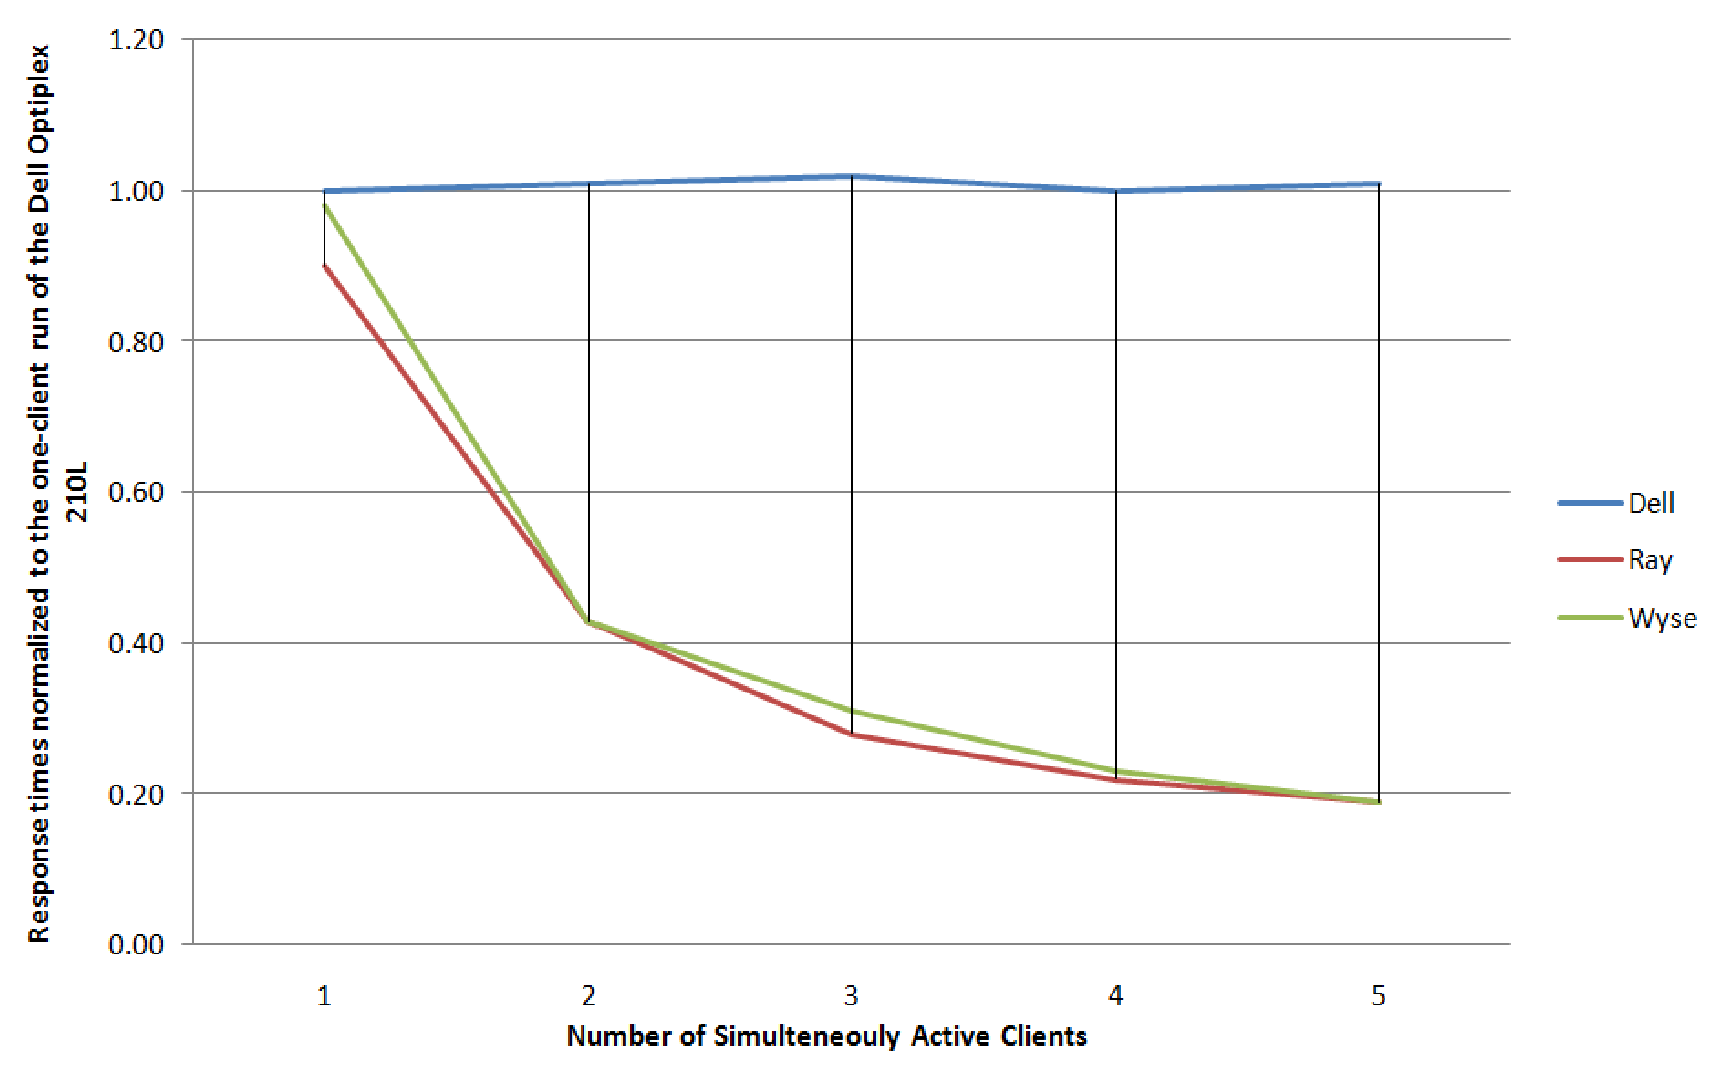
\includegraphics{graphics/graphic_excel_test}}
                    \caption{Normalized Excel Subtotals Task Response Times}
                    \label{fig:graphic_excel_test}
                \end{figure}
                \begin{table}[h!tb]
                    \centering
                    \begin{tabular}{|c|c|c|c|c|c|c|}
                    \hline
                    \multicolumn{ 3}{|c|}{Performance Results} &            & \multicolumn{ 3}{|c|}{Comparative Rating} \tnhl
                    PC solution & \multicolumn{ 2}{|c|}{Thin-client solutions} & Number of   & PC solution & \multicolumn{ 2}{|c|}{Thin-client solutions} \tnhl
                          Dell &        Sun &       Wyse & concurrent &       Dell &        Sun &       Wyse \tn

                      OptiPlex &        Ray &    Winterm &     active &   OptiPlex &        Ray &    Winterm \tn

                          210L &          2 &     5150SE &    clients &       210L &          2 &     5150SE \tnhl
                          12.9 &       13.2 &       13.1 &          1 &       1.00 &       0.90 &       0.98 \tnhl
                          12.8 &       30.2 &       29.7 &          2 &       1.01 &       0.43 &       0.43 \tnhl
                          12.7 &       45.5 &       41.9 &          3 &       1.02 &       0.28 &       0.31 \tnhl
                          12.9 &       58.3 &       57.3 &          4 &       1.00 &       0.22 &       0.23 \tnhl
                          12.8 &       68.1 &       67.9 &          5 &       1.01 &       0.19 &       0.19 \tnhl
                    \end{tabular}  
                    \captionof{table}{Performance Results for Excel Subtotals Calculation} 
                    \label{tab:table_excel_test}
                \end{table}
                \begin{figure}[h!tb]
                    \centering
                    \resizebox{\textwidth}{!}{ % Fazendo a tabela caber no espaco da pagina
                    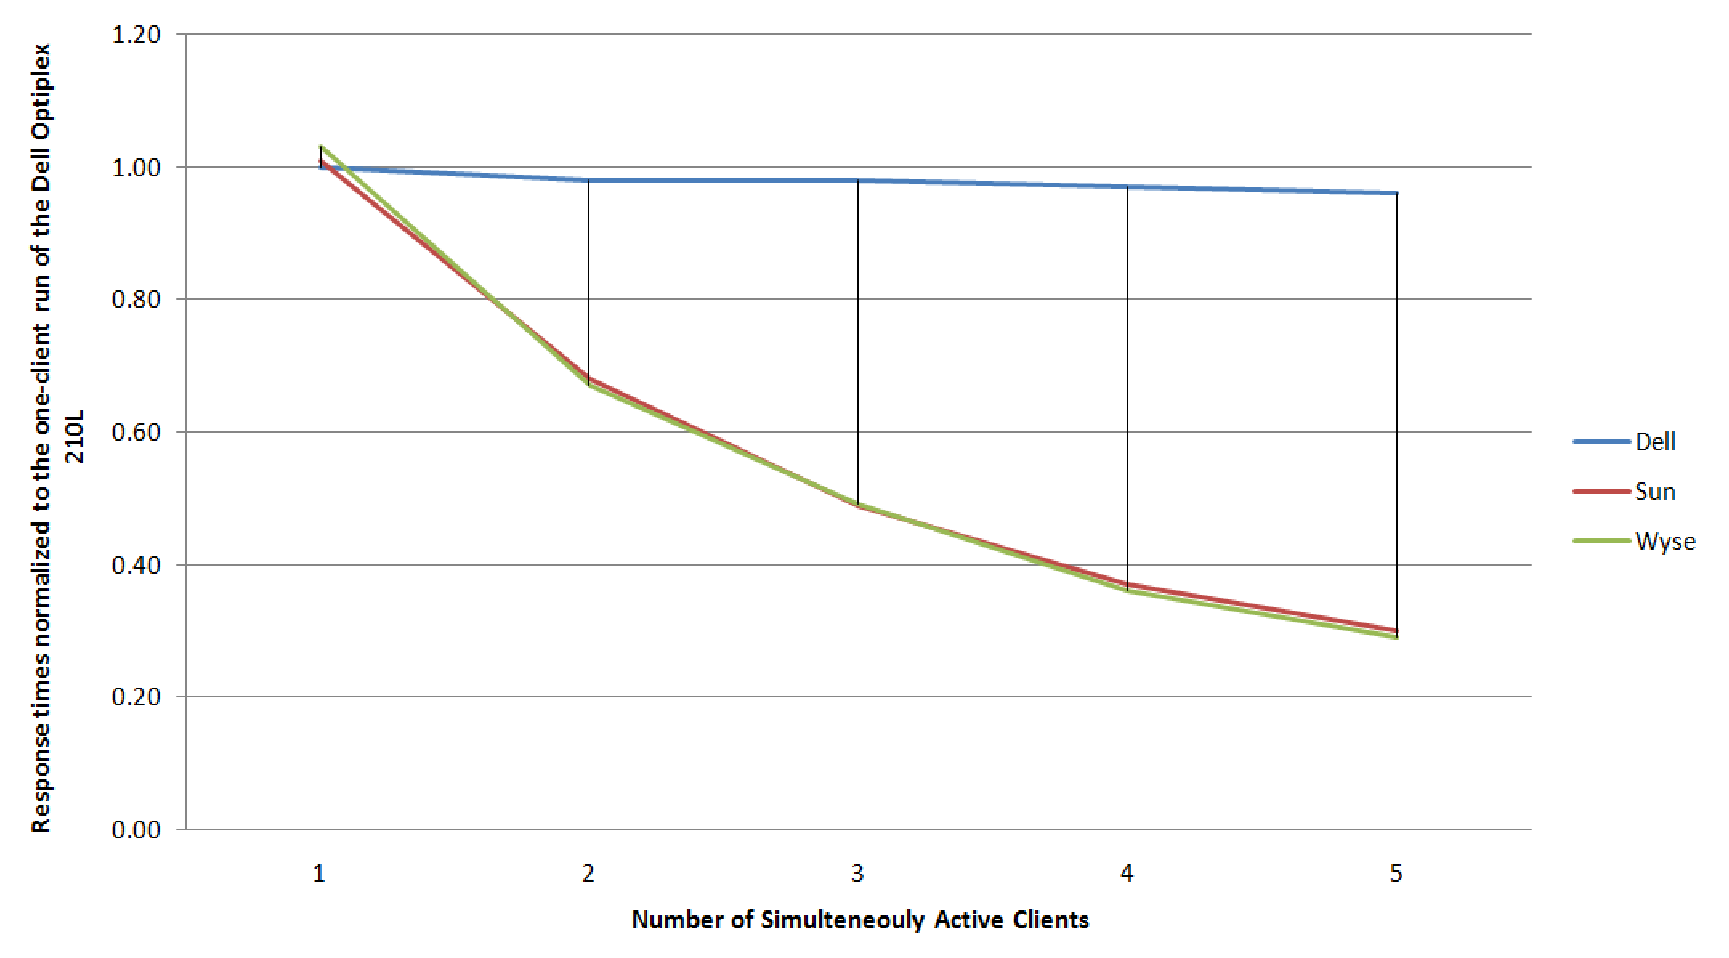
\includegraphics{graphics/graphic_pdf_test}}
                    \caption{Normalized PDF Subtotals Task Response Times}
                    \label{fig:graphic_pdf_test}
                \end{figure}
                \begin{table}[h!tb]
                    \centering
                    \begin{tabular}{|c|c|c|c|c|c|c|}
                    \hline
                    \multicolumn{ 3}{|c|}{Performance Results} &            & \multicolumn{ 3}{|c|}{Comparative Rating} \tnhl
                    PC solution & \multicolumn{ 2}{|c|}{Thin-client solutions} & Number of   & PC solution & \multicolumn{ 2}{|c|}{Thin-client solutions} \tnhl
                        Dell   &        Sun &       Wyse & concurrent &     Dell   &        Sun &       Wyse \tn

                      OptiPlex &        Ray &    Winterm &     active &   OptiPlex &        Ray &    Winterm \tn

                          210L &          2 &     5150SE &    clients &       210L &          2 &     5150SE \tnhl
                          16.1 &       16.0 &       15.6 &          1 &       1.00 &       1.01 &       1.03 \tnhl
                          16.4 &       23.8 &         24 &          2 &       0.98 &       0.68 &       0.67 \tnhl
                          16.5 &       33.0 &       33.1 &          3 &       0.98 &       0.49 &       0.49 \tnhl
                          16.6 &       43.7 &       44.3 &          4 &       0.97 &       0.37 &       0.36 \tnhl
                          16.7 &       54.0 &       55.1 &          5 &       0.96 &       0.30 &       0.29 \tnhl
                    \end{tabular}  
                    \captionof{table}{Performance Results for PDF Compression Subtotals Calculation}
                    \label{tab:table_pdf_test}
                \end{table}
                \pagebreak
            \subsubsection*{PC vs. Thin Client: Power Consumption}
                Supposing 30 thin users share a 400W server, the total power consumption will be 1300W - a yearly cost of \euro640.00. 30 PCs would consume 10000W instead - a yearly cost of \euro4900.00 (assuming the MWh cost is \euro80.00). The Table~\ref{tab:pc_thin_client_power_consumption} shows the power consumption of thin-client and PC.
                \begin{table}[h!tb]
                \centering
                    \begin{tabular}{|c|c|c|}
                    \hline
                         & {\bf Thin Client} &   {\bf PC} \tnhl
                    {\bf Weight} & 2.2 - 7.7 lbs & 22 - 33 lbs \tnhl
                    {\bf Volume} & 1.5 - 3 dm$^3$ & 30 - 35 dm$^3$ \tnhl
                    {\bf Packing material} & 2.2 - 4.4 lbs &   3 - 5 kg \tnhl
                    {\bf Power consumption\linebreak (including monitor)} & 20 - 50 watt & 300 - 400 watt \tnhl
                    {\bf Heat rejection} & 5 - 35 watt & 85 - 115 watt \tnhl
                    {\bf Noise level} & 0 dbA & 50 - 60 dbA \tnhl
                    \end{tabular}  
                    \captionof{table}{PC and thin client power consumption} 
                    \label{tab:pc_thin_client_power_consumption}
                \end{table}
                
            \subsubsection*{Hardware Savings}
                \paragraph*{Savings on client hardware} 
                    The economy brought by the substitution of PCs with thin clients was estimated around US\$ 208 per PC per year. The estimative considered the average prices of a PC, an adequate thin client and the PC upgrade costs every 3 years. If energy consumption is considered, the savings will be even greater.

                The following considerations were taken:
                \begin{itemize}
                    \item Thin client cost: US\$250.00 x PC cost: US\$750.00;
                    \item PC needs to be upgraded every 3 years and thin clients need to be replaced every 6 years.
                \end{itemize}
                Therefore, in a 6-year period US\$1500.00 will be spent on a PC against US\$250.00 that will be spent on a thin client.

            \paragraph*{Extra server hardware costs}
                Considering that:
                \begin{itemize}
                    \item On average 30 users will need a dual processor server with 4 GB of RAM and SCSI hard disks;
                    \item A brand new server should cost around US\$4,500.00 and will depreciate on average in 3 years.
                \end{itemize}
                For 60 users, the thin client solution should out-price the PC one by US\$11,300.00 per year, excluding the administration costs of both solutions.

        \subsection{Servers and Virtualization} \label{sec2:servers_virtualization}
                        
            \subsubsection*{Rack vs. Blade}
                According to Goldworm\cite{barbAnne07}, Blade servers are a package of ``ultra-high density components including servers, storage, and communications interfaces in a pre-wired chassis with shared components such as power, cooling, and networking. In contrast to the conventional \emph{horizontal} positioning within a rack (rack mounted servers), blades servers are typically (though not always) installed \emph{vertically} in a blade chassis, like books in a bookshelf''. This disposition of the blade servers along with their reduced dimension provide a high server density and thus of performance. For example, 60 blade servers such as the one depicted in Figure~\ref{fig:example_blade_server} can fit in the same physical space as 42 rack-mounted servers. A blade enclosure, which can hold from 8 to 24 \cite{Rehn08} blade servers, provides common services such as power supply, cooling and networking thus eliminating redundancies in each individual blade server. A standard rack can accommodate more than 250 blade servers against approximately 42 standard servers.
            \begin{figure}[h!tb]
                \centering
                \subfloat[IBM LS20]{
                    \label{fig:ibm_ls20_blade_server}
                    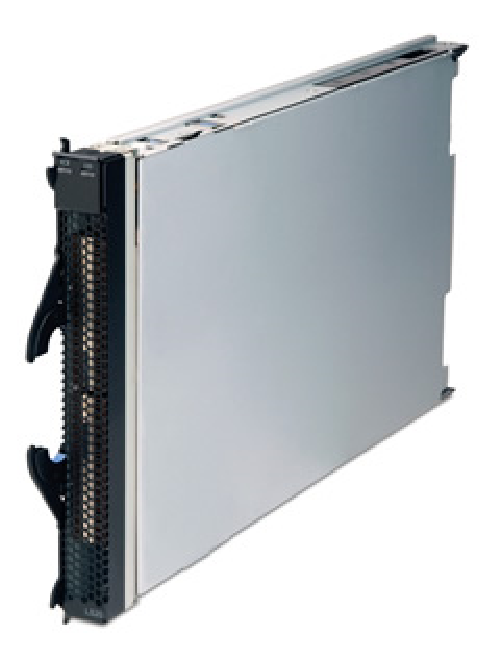
\includegraphics[width=0.3\textwidth]{graphics/ibm_ls20_blade_server}}
                \subfloat[Sun 6000 Series Blade Enclosure]{
                    \label{fig:sun_6000_blade_enclosure}
                    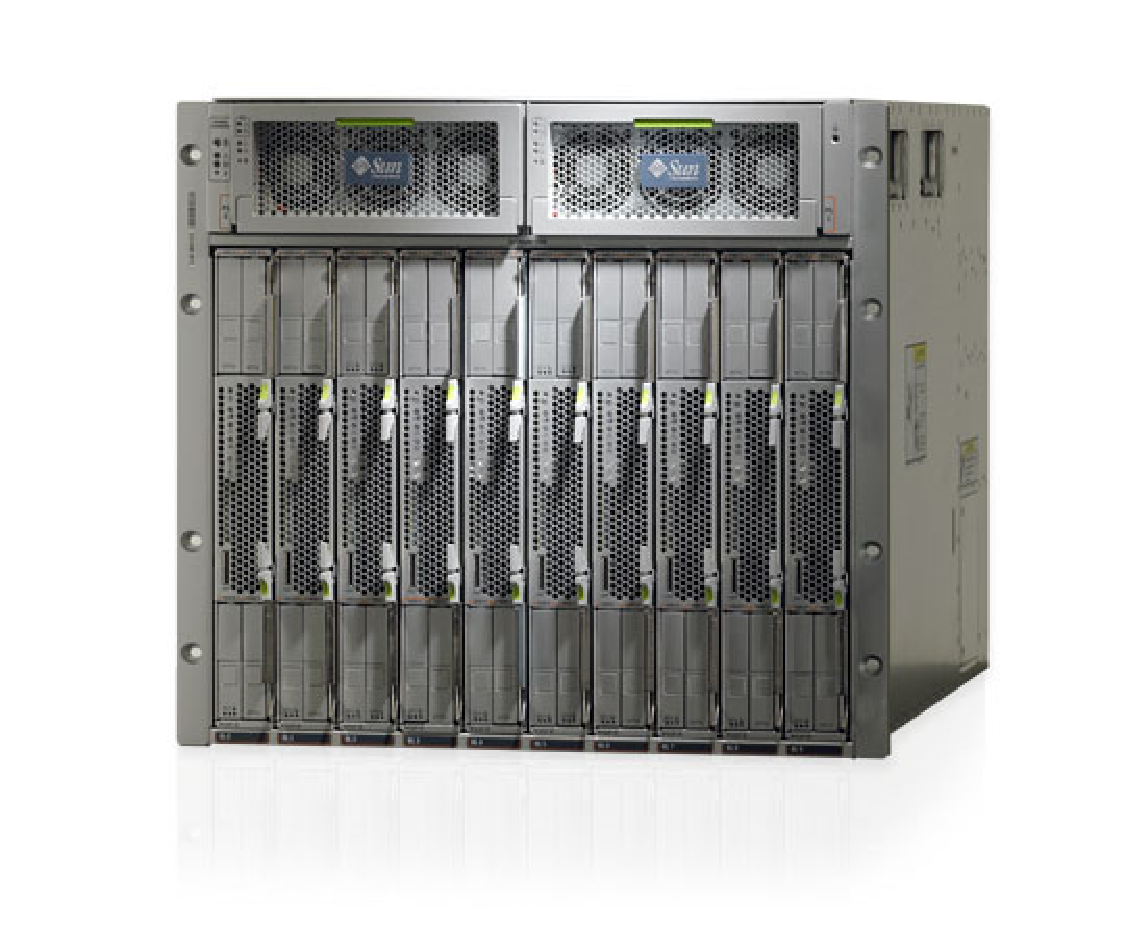
\includegraphics[width=0.3\textwidth]{graphics/sun_6000_blade_enclosure}}
                \subfloat[HP Intros Rack]{
                    \label{fig:hp_intros_blade_server_rack}
                    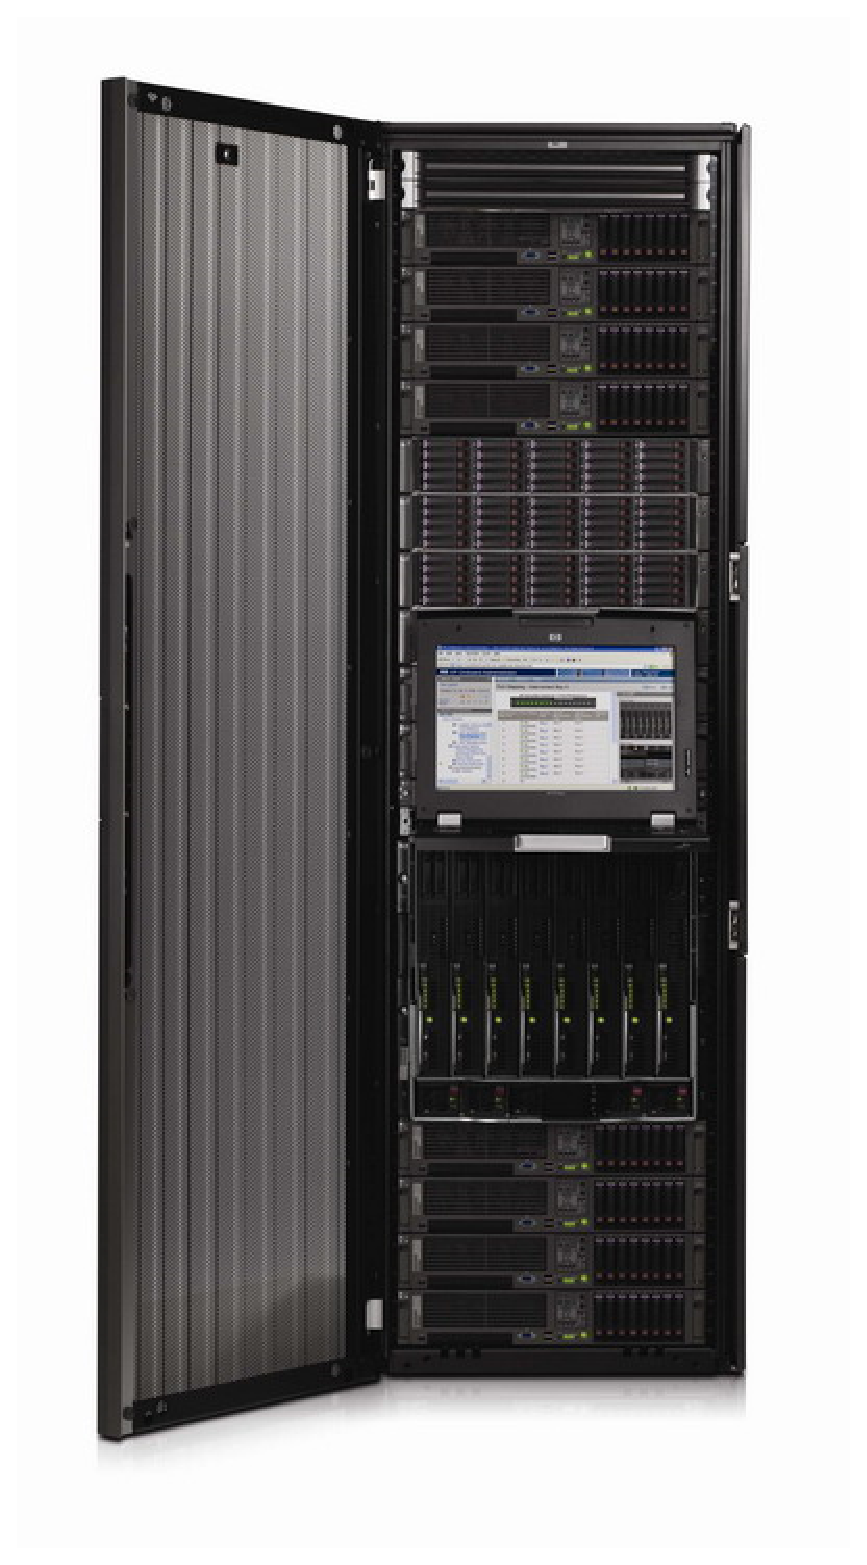
\includegraphics[width=0.3\textwidth]{graphics/hp_intros_blade_server_rack}}
                \caption{Examples of Blade Servers}
                \label{fig:example_blade_server}
            \end{figure}
            \begin{figure}[h!tb]
                \centering
                \subfloat[Chenbro 5U RM51924]{
                    \label{fig:chenbro_5urm51924}
                    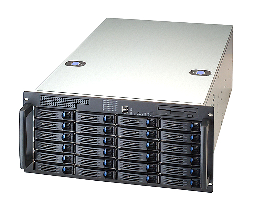
\includegraphics[width=0.3\textwidth]{graphics/chenbro_5U_RM51924}}
                \subfloat[Rack Server]{
                    \label{fig:rack_server}
                    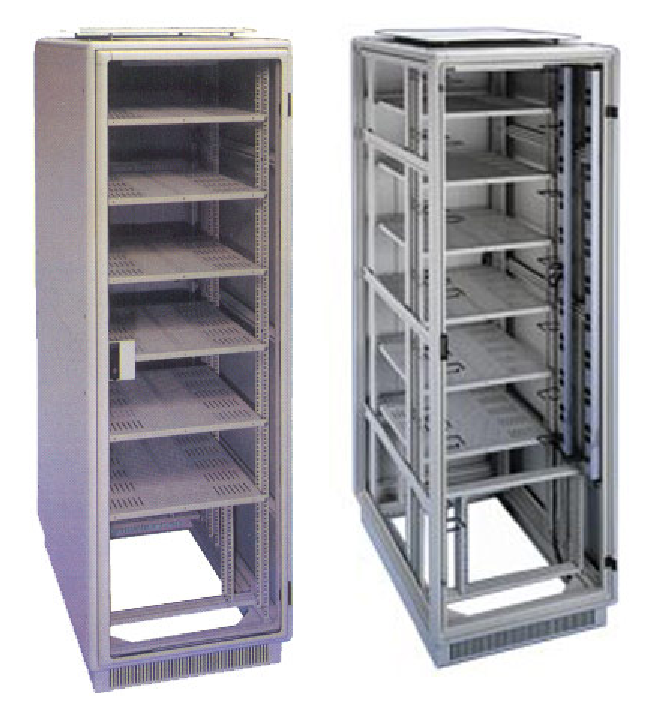
\includegraphics[width=0.3\textwidth]{graphics/rack_server}}
                \caption{Examples of Rack Servers}
                \label{fig:example_rack_server}
            \end{figure}
            In the Table~\ref{tab:power_consumption_several_servers}, a comparison is made between IBM HS21 blades and x3550 rack servers. The blades and rack servers have comparable performance.
            \begin{itemize}
                \item 2.0 GHz intel quad core;
                \item 8 GB DDR2 memory;
                \item Both in standard configuration, with no HDDs.
            \end{itemize}
            \begin{table}[h!tb]
                \centering
                \begin{tabular}{|c|c|c|c|}
                \hline
                \multicolumn{ 1}{|c|}{{\bf IBM server model}} & \multicolumn{ 1}{|c|}{{\bf Base Power}} & \multicolumn{ 1}{|c|}{{\bf kWh consumed}} & \multicolumn{ 1}{|c|}{{\bf Total cost }} \tn
                \multicolumn{ 1}{|c|}{{\bf }} & \multicolumn{ 1}{|c|}{{\bf Consumption}} & \multicolumn{ 1}{|c|}{{\bf over 5 years}} & \multicolumn{ 1}{|c|}{{\bf (\$0.03/kWh)}} \tn
                \multicolumn{ 1}{|c|}{{\bf }} & \multicolumn{ 1}{|c|}{{\bf }} & \multicolumn{ 1}{|c|}{{\bf }} & \multicolumn{ 1}{|c|}{{\bf over 5 years}} \tnhl
                BC-H Chassis, no blades & 0.510 kWh &     22,350 &  \$670.50  \tnhl
                BC-H HS21 blade & 0.318 kWh &     13,936 &  \$418.08  \tnhl
                x3550 server & 0.373 kWh &     16,346 &  \$490.39  \tnhl
                x3650 server & 0.455 kWh &     19,940 &  \$598.20  \tnhl
                BC-H chassis with 14 & 4.962 kWh &    217,455 & \$6,523.65  \tn
                HS21 blades &  &  &  \tnhl
                14 x3550 servers & 5.222 kWh &    228,849 & \$6,865.46 \tnhl
                14 x3650 servers & 6.370 kWh &    279,259 & \$8,374.80  \tnhl
                \end{tabular}  
                \captionof{table}{Power consumption for several servers, excluding cooling and redundancy}%XXX colocar referencia
                \label{tab:power_consumption_several_servers}
            \end{table}

            \begin{itemize}
                \item Space saving and efficiency - packing more computer power in a significantly smaller area;
                \item Consolidation of servers to improve and centralize management as well as utilization;
                \item Return on investment (ROI) and improved total cost of ownership (TOC) through increased hardware utilization and reduced operating expenses;
                \item More energy efficient, due to existence of centralized power supply, cooling and networking.
            \end{itemize}
            According to the figures, the choice of using a blade server provides roughly 5\% power saving over a similar rack-mount configuration. The main benefit brought by the use of blade servers, however, is the processing density, as a rack filled with blade servers may carry up to 50\% more servers than one with rackable servers. Other benefits are that blade servers are easier to service and reduce the number of power cables needed from as much as 80\% \cite{Hendenson07}. 
            
            In conclusion, blade servers do not provide much in terms of power saving but it greatly reduces the amount of space used in datacenters. However, the high power density might prove to be a problem to server farms in terms of overheating. Solutions to this problem are described in the section of Data Center Infrastructure.
            
            \subsubsection*{Virtualization}
                The overall goal of virtualization is to create a logical abstraction of physical assets. It allows multiple ``virtual'' servers to run on one physical server, thereby consolidating many physical servers into one. \emph{Wikipedia}, in 2009, defines virtualization as the following: ``Virtualization is the process of presenting a logical grouping or subset of computing resources so that they can be accessed in ways that give benefits over the original configuration. This new virtual \emph{view} of the resources is not restricted by the implementation, geographic location or the physical configuration of underlying resources.''. Virtualization can improve efficiency and availability of resources and applications in the organization and according to \emph{Vmware}, the choice of virtualized servers over the standard nonvirtualized configuration makes possible to save 50-70\% overall IT costs. Apart from the reduction of costs, virtualization may free up IT resources, provide better infrastructure optimization and utilization, increase availability and improve desktop management.
                
                Besides that, virtualization has made positive improvements to the environment issue. Gartner \cite{GartnetStamford07} estimates that 1.2 million workloads run in virtual machines, which represents an annual aggregate power savings of about 8.5 billion kWh - more electricity than is consumed annually in all of New England for heating, ventilation and cooling. While this is a good start, there are plenty of opportunities for saving even more energy and money. Analyst firm IDC \cite{IDCDoc07} states that the un-utilized server capacity equates to approximately:
                \begin{itemize}
                    \item in term of equipment and energy costs : US\$140 billion annually
                    \item in terms of hardware costs : 3 years supply of hardware
                    \item in terms of computing power : more than 20 million servers 
                \end{itemize}
                At the annual production rate of 4 tons of carbon dioxide (CO$_{2}$) per server, these un-utilized servers produce a total of more than 80 million tons of CO$_{2}$ per year. This is more than is emitted from the country of Thailand and more than half of all countries in South America. From the organizational point of view these data suggests that virtualization is a good improvement to the data center, saving not only space provided to the servers but also saving energy by reducing the idle time of the servers and augmenting their workload. It is also important to state that, by providing a virtualized solution, the number and variety of available applications can be increased.
                
                There are two kinds of virtualization that may be used in a data center: storage and computing virtualization. Storage-area networks (SAN) may be implemented to present several different physical storage racks as a single virtual storage pool \cite{Antonopoulos05}. On the other hand, computing virtualization can be implemented in two ways. The first case is when a single physical server can offer multiple virtual servers, each with its own OS. Another option is to consolidate multiple physical servers into a cluster that acts as a single server. There are cross-platform server virtualization softwares available which allows data center managers to cluster and partition servers.
                \begin{figure}[h!tb]
                    \centering
                    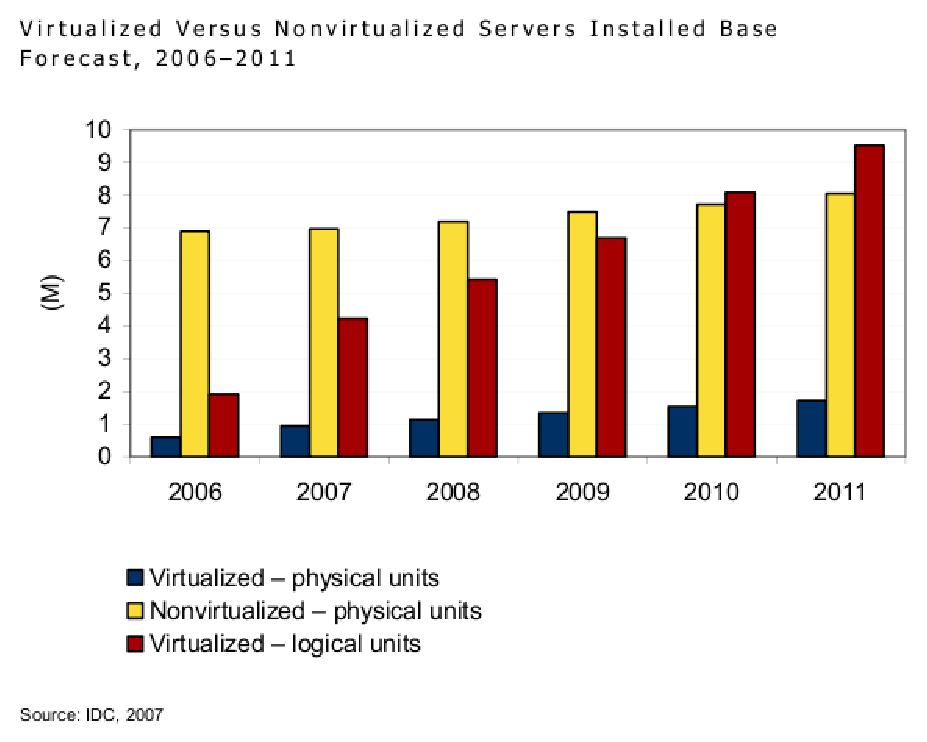
\includegraphics{graphics/installed_base_virtualized_servers}
                    \caption{Installed Base of Virtualized and Non-Virtualized Servers}
                    \label{fig:installed_base_virtualized_servers}
                \end{figure}
                
                According to the Figure~\ref{fig:installed_base_virtualized_servers} there is a trend indicating an increasing number of virtualized units over time along a forecast that by the end of 2009 the number of virtualized servers will be greater than non-virtualized ones. Logical units represent virtualized storage while physical units represent the use of non-virtualized storage. As shown in the Figure~\ref{fig:illustration_virtualization_to_physical_server}, virtualization tools such as VMware allow one physical server to act as a number of logical servers. VMware also provides a benchmark tool called VMmark\footnote{\url{http://www.vmware.com/products/vmmark/}} along with a set of test results in \cite{Makhija06} for a configuration that includes a mail server, a java server, a standby server, a web server, a database server and a file server.
                \begin{figure}[h!tb]
                    \centering
                    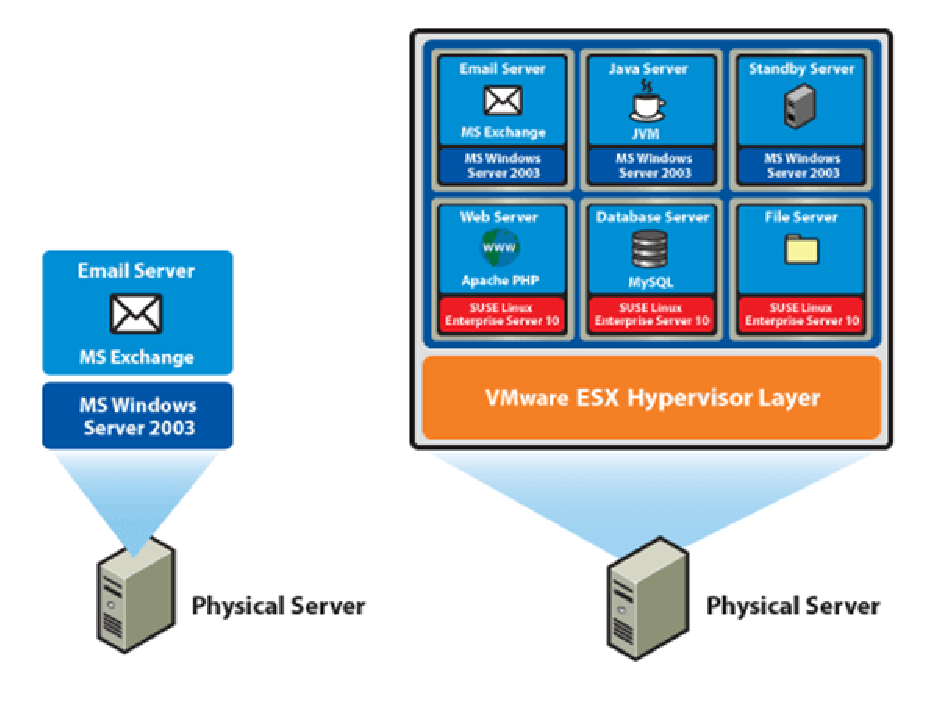
\includegraphics[scale=0.7]{graphics/illustration_virtualization_to_physical_server}
                    \caption{Illustration of Virtualization Applied to a Physical Server}
                    \label{fig:illustration_virtualization_to_physical_server}
                \end{figure}
                
                Coming along with the virtualization trend are high-throughput and eco-responsible processors such as the Sun's UltraSPARC T1 processor \cite{Hetherington05}, which support up to 128 virtualized systems in a single server and gives one of the best performance per watt of the available processors. As shown in the Table~\ref{tab:performance_power_dissipation_several_processors}\footnote{\url{http://www.anandtech.com/cpuchipsets/showdoc.aspx?i=2657&p=4}}, with relation to the UltraSPARC CPU the only comparable performance was met by the POWER5+ processor, which in average dissipates 4.5 times as much as the earlier.
                \begin{table}[h!tb]
                    \centering
                    \begin{tabular}{|c|c|c|c|c|c|c|}
                    \hline
                          &            & {\bf Power}       &                & {\bf Number}  &           &  \tn
                        &            & {\bf Dissipation} &                & {\bf of}      &           &  \tn
                        &            & {\bf CPUs}        & {\bf Number}   & {\bf Active}  & {\bf Score}   & {\bf Score} \tn
                  {\bf System} & {\bf CPU} & {\bf (Estimated)} & {\bf of cores} & {\bf Threads} & {\bf (bops)} & {\bf (\%)} \tnhl
                    Sun Fire  &  1x 1.2GHz &    72-79 W &          8 &         32 &     63.378 &      160\% \tn
                    T2000 & UltraSPARC T1 &            &            &            &            &            \tnhl
                    Sun Fire  &  2x 2.4GHz &  150-180 W &          4 &          4 &     45.124 &      114\% \tn
                    X4200 & DC Opteron &            &            &            &            &            \tnhl
                    IBM &  2x 1.9GHz &  320-360 W &          4 &          8 &     61.789 &      156\% \tn
                    p5 550 &    POWER5+ &            &            &            &            &            \tnhl
                    IBM 346 & 2x 2.8GHz  &  270-300 W &          4 &          8 &     39.585 &      100\% \tn
                    xSeries &    DC Xeon &            &            &            &            &            \tnhl
                    \end{tabular}
                    \captionof{table}{Performance and Power Dissipation for Several Processors by the Specjbb2005 Java Benchmark}
                    \label{tab:performance_power_dissipation_several_processors}
                \end{table}
                
        \subsection{Data Storage} \label{sec2:data_storage}
            There are currently three main technologies to store data: hard disks, tape drives and flash-based storage. This session will cover the first two, as they are the predominant technologies in datacenters. At the end of the session a comparison will be made between hard and tape drives.
            
            \subsubsection*{Tape Drives}
                A tape drive is a data storage device that reads and writes data stored on a magnetic tape. Its main use is as archival storage of data stored in hard drives. It is typically used for archival storage of data stored on hard drives. 
Tape media generally has a favorable unit cost, long archival stability and low energy consumption per MB of data stored to compensate for their slow seek times. Despite the slow seek time, tape drives can stream data to tape as quickly as hard drives. For example, modern LTO drives can reach continuous data transfer rates of up to 80MB/s, which is as fast as most 10,000rpm hard disks, according to \emph{Wikipedia, 2008}. Tape drives can range in capacity from a few megabytes to hundreds of gigabytes. Data can be compressed as to maximize the capacity usage. In this case the compression rate is of usually 2:1. A set of tables related to tape drives can be found in Appendix~\ref{app:comparison_tape_drives}
            
            \subsubsection*{Disk Arrays}
                Disk array refers to a linked group of one or more physical independent hard disks constituting a larger, high-performance system. They are usually implemented using RAID technology, which can provide component redundancy and high throughputs.
        
            \subsubsection*{Comparison between Tape Drives and Disk Arrays}
                Supposing a 995 TB database consisting of:
                \begin{itemize}
                	\item Storage base (frequently used data)
                	\item Backup cache (13 weeks)
                	\item Backup archive (1 year backup)
                \end{itemize}
                A solution consisting exclusively of disk arrays would require four 32-drawer disk array systems of 245 TB each. In order to ensure reliability and recoverability, a RAID5 format with two RAID5 arrays assigned to each drawer has been assumed. The total equipment cost is estimated on US\$10.57M \cite{Reine08} and according to the following table the disk array solution consumes 98KWh per TB per year.
                \begin{table}[h!tb]
                \centering 
                \resizebox{\textwidth}{!}{ % Fazendo a tabela caber no espaco da pagina
                \begin{tabular}{|c|c|c|c|c|c|c|c|c|}
                \hline
                & & {\bf Standby} & {\bf Per} & {\bf Number} & {\bf Total} & {\bf Power} &  & {\bf Annual} \tn
                & {\bf Processor} & {\bf Power} & {\bf SATA} & {\bf of SATA} & {\bf Array} &  {\bf Per} & {\bf Annual} & {\bf Cost} \tn
                {\bf Power} & {\bf Chassis} & {\bf Supply} & {\bf Drawer} & {\bf Drawers} & {\bf Power} &  {\bf Day} & {\bf Power} & US\$0.12/kWh \tnhl
                {\bf Typical} &  430 W/h &  34 W/h &  325 W/h &   32 &  11 kW/h & 264 kWh & 96,360 kWh & 11,563 \tnhl
                {\bf Maximum} &  800 W/h &  300 W/h &  425 W/h &   32 &  15 kW/h & 360 kWh & 131,400 kWh &  15,768 \tnhl
                \end{tabular}}
                \captionof{table}{Tape Drive Power Costs}%XXX verificar nome da tabela
                \label{tab:tape_drive_power_costs} %XXX verificar nome da tabela
                \end{table}
                With a native capacity of 800GB and throughput of 120 MB/sec, an LTO 4 drive has a compressed capability to write at 240 MB/sec, or 864 GB/hour. Supposing the same database is to be entirely stored at this drive, the equipment cost would be of US\$233,878.00 with an annual energy cost of US\$599.00.The tape solution will consume 1150 kWh in 1 year or 1,16kWh per TB per year.
                \begin{table}[h!tb]
                \centering 
                \resizebox{\textwidth}{!}{ % Fazendo a tabela caber no espaco da pagina
                \begin{tabular}{|c|c|c|c|c|c|c|c|c|}\hline
                {\bf N$^o$ of  } & {\bf N$^o$ of } & {\bf Library } & {\bf Frame} & & {\bf Drive} &  &   &  \tn
                {\bf frames} & {\bf drives } & {\bf acquisition } & {\bf acquisition } & {\bf Cartridge } & {\bf acquisition } & {\bf Space} & {\bf Energy} & {\bf Total} \tn
                {\bf acquired} & {\bf acquired} & {\bf cost} & {\bf cost} & {\bf cost} & {\bf cost} & {\bf cost} & {\bf cost} & {\bf cost} \tnhl
                1 &    2 &    76,000 &    30,000 &   82,278 &   45,600 &   68,850 &   599 &    303,327 \tnhl
                \end{tabular}}
                \captionof{table}{Disk Array Power Costs}%XXX verificar nome da tabela
                \label{tab:disk_array_power_costs} %XXX verificar nome da tabela
                \end{table}
                In overall, for the 995 TB database the following conclusions can be drawn:
                \begin{itemize}
	                \item Disk arrays consume 84 times as much as tape drives, per TB stored
	                \item The disk array solution costs 35 times as much as the tape drive solution
                \end{itemize}
                Although the cost difference between of both solutions may be high, performance should be also considered in the comparison. In that case, an adequate proportion between disk array and tape storage must be drawn according to the frequency of backup access.

        \subsection{Power Architectures} \label{sec2:power_architectures}
            \subsubsection*{Conventional AC Architecture}
                \begin{figure}[h!tb]
                    \centering
                    \resizebox{\textwidth}{!}{ % Fazendo a tabela caber no espaco da pagina
                    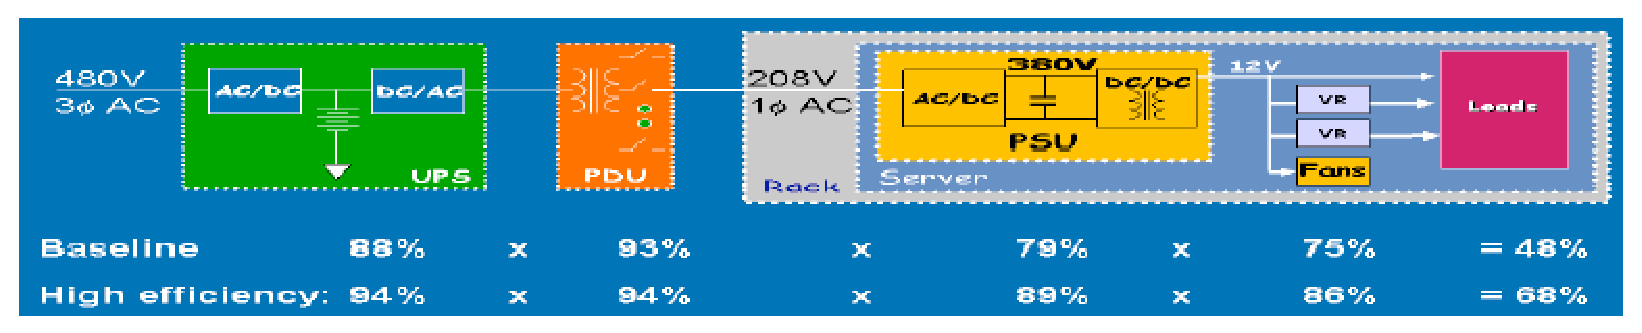
\includegraphics{graphics/conventional_ac_efficiency}}
                    \caption{Conventional AC architecture efficiency}
                    \label{fig:conventional_ac_efficiency}
                \end{figure}
                In this configuration (Figure~\ref{fig:conventional_ac_efficiency}) the following transformations take place:
                \begin{itemize}
	                \item PDU steps down the voltage from 480VAC to 208VAC;
                    \item Power Supply Unit (PSU) converts 208VAC to 380VDC;
                    \item Final component distribution at 12VDC.
                \end{itemize}
                The efficiency is measured for both conventional (baseline) and high efficiency (best-in-class) equipments. The difference in efficiency between the two equipment choices is of 20\%.

            \subsubsection*{Rack-Level DC Architecture}
                \begin{figure}[h!tb]
                    \centering
                    \resizebox{\textwidth}{!}{ % Fazendo a tabela caber no espaco da pagina
                    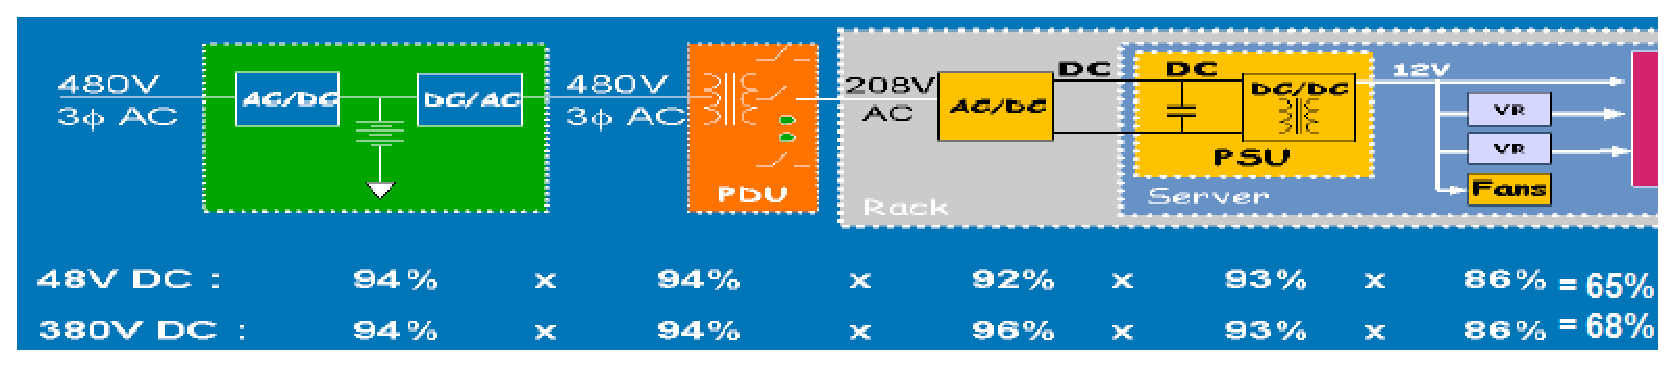
\includegraphics{graphics/rack_level_dc_efficiency}}
                    \caption{Rack-level DC architecture efficiency}
                    \label{fig:rack_level_dc_efficiency}
                \end{figure}
                On Figure~\ref{fig:rack_level_dc_efficiency}, it is possible to see that, after the PDU, an 208VAC to 48VDC/380VDC conversion is made in the rack. PSU and PDU are considered to be best-in-class, with high efficiency.

            \subsubsection*{Facility-level DC Architecture}
                \begin{figure}[h!tb]
                    \centering
                    \resizebox{\textwidth}{!}{ % Fazendo a tabela caber no espaco da pagina
                    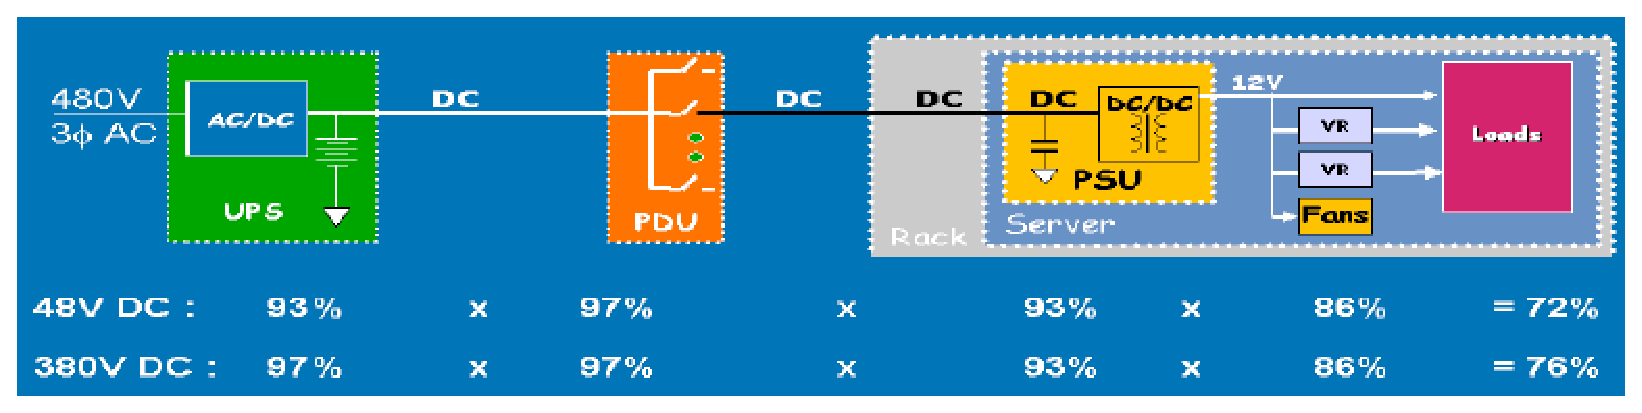
\includegraphics{graphics/facility_level_dc_efficiency}}
                    \caption{Facility-level DC architecture efficiency}
                    \label{fig:facility_level_dc_efficiency}
                \end{figure}
                In this configuration (Figure~\ref{fig:facility_level_dc_efficiency}), the DC-AC conversion in the UPS and the AC-DC conversion in the power supply are removed. It can be noted that the 480VAC-380VDC conversion in the UPS is more efficient than the 480VAC-48VDC conversion.
            
        \subsection{Data Center Infrastructure} \label{sec2:data_center_infrastructure}
            \subsubsection*{Water Cooling}
                The reasonable limit of rack power and cooling capacity for a conventional forced-air (HVAC) cooled data center is 8 kW per rack. For power densities approaching 15 kW per rack, the layout of the computing rooms and cooling facilities must be determined using specialized software (such as HP Static Smart Cooling). For racks requiring more than 15 kW, the latest cooling techniques use water (Figure~\ref{fig:power_consumption_number_servers_rack}) \cite{HPCooling07}.
                \begin{figure}[h!tb]
                    \centering
                    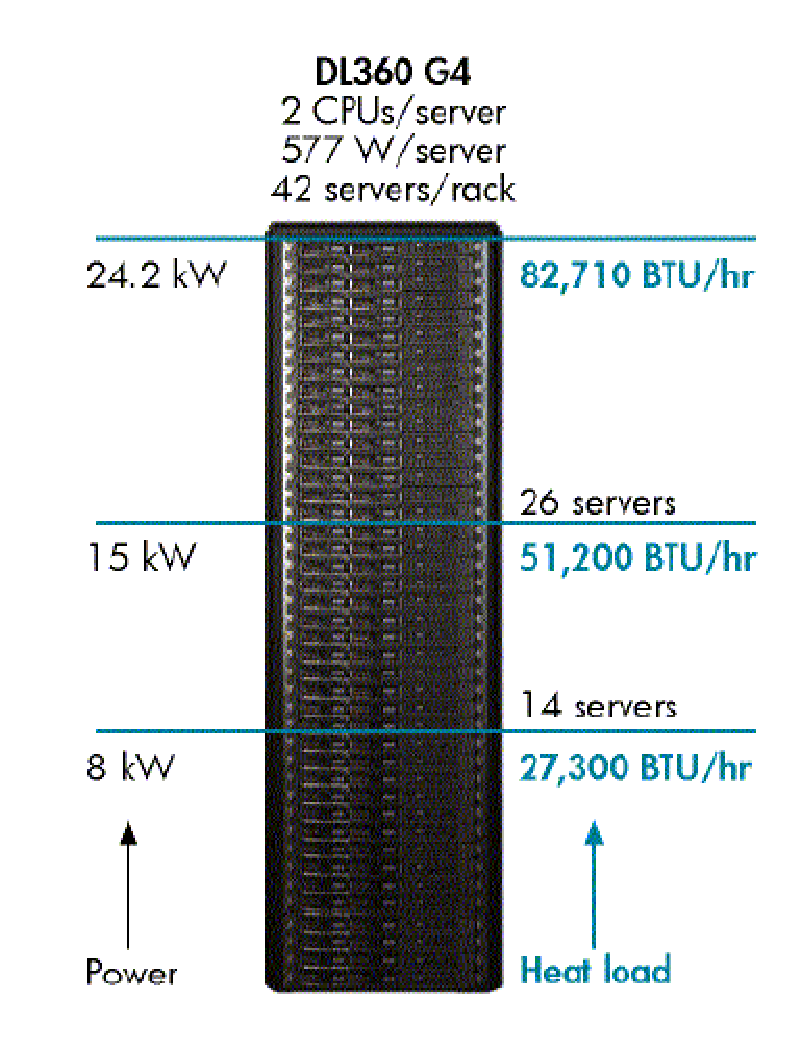
\includegraphics[scale=0.5]{graphics/power_consumption_number_servers_rack}
                    \caption{Power Consumption per Number of Servers in the Rack}
                    \label{fig:power_consumption_number_servers_rack}
                \end{figure}
                As shown in the following figure, the use of water cooling reduces in 50\% the equipment footprint, allowing greater server density. A 35 kW heat load dispersed among 4 racks could be concentrated in one single rack.
                \begin{figure}[h!tb]
                    \centering
                    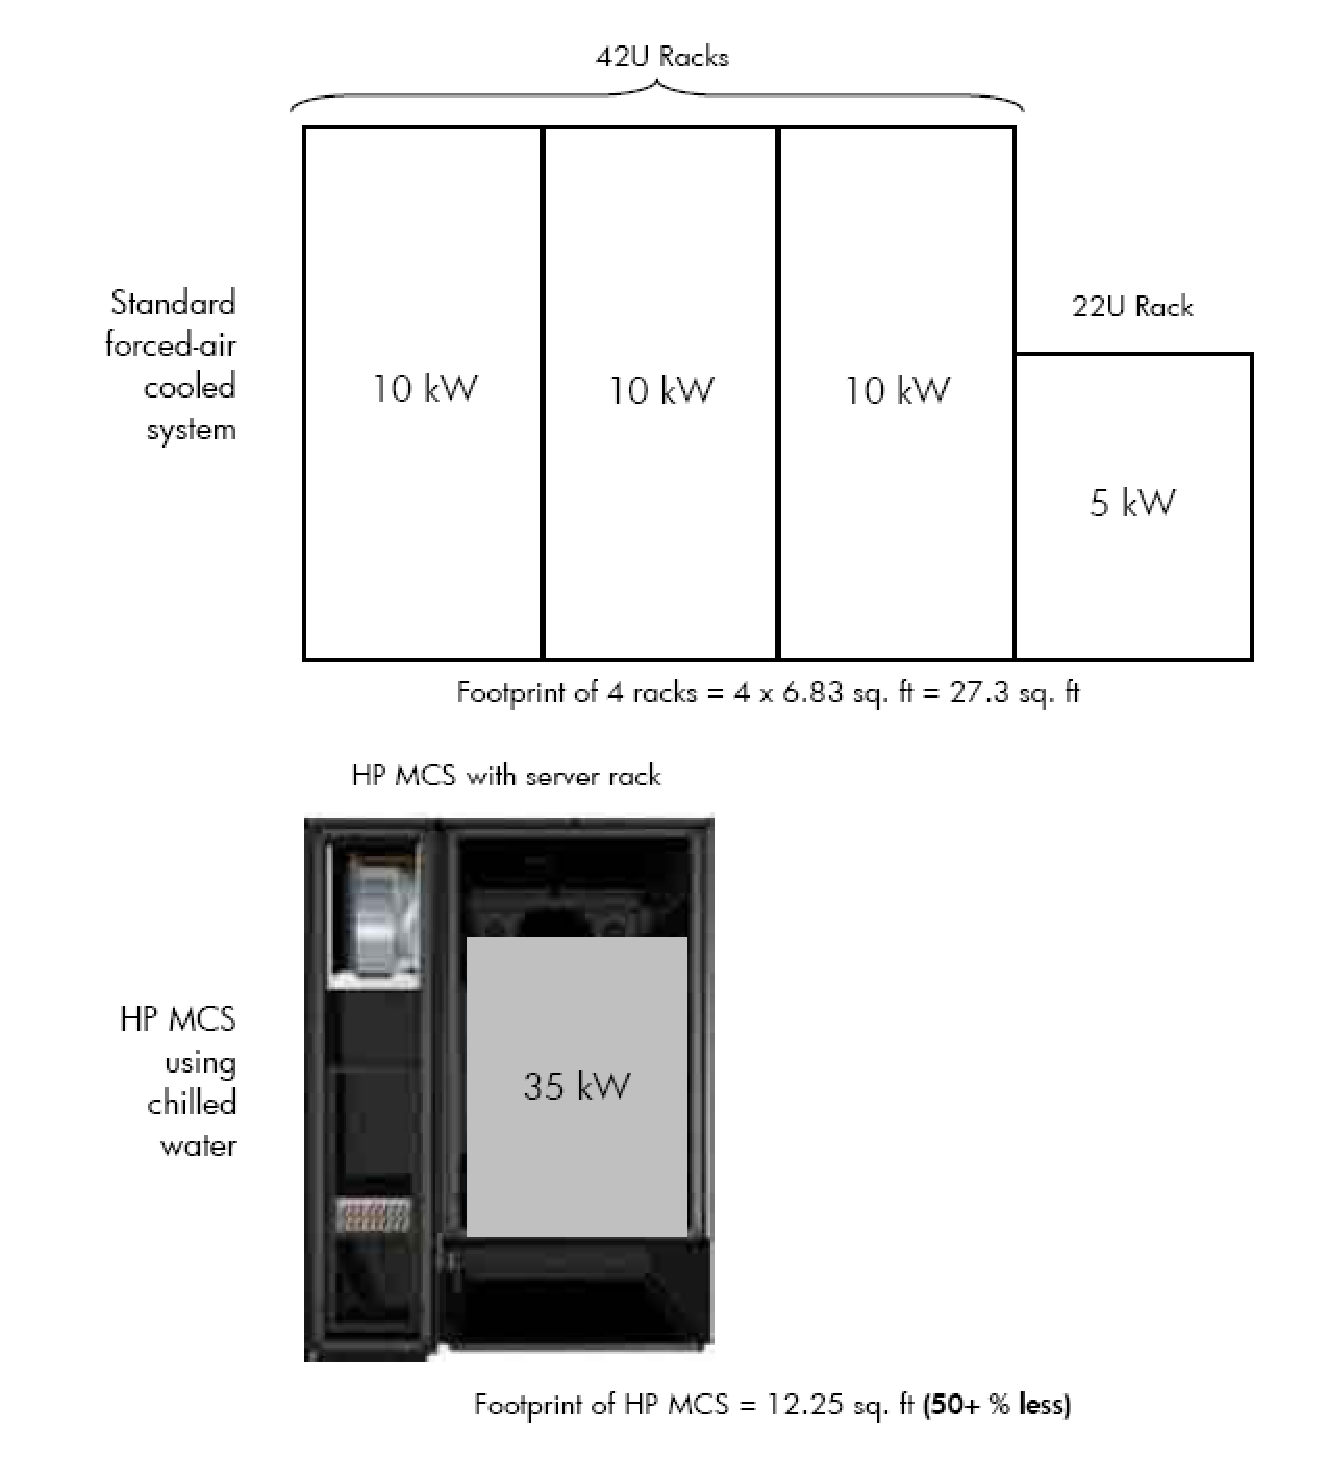
\includegraphics[scale=0.5]{graphics/footprint_reduction_for_35_heat_load}
                    \caption{Footprint Reduction for a 35 kW Heat Load}
                    \label{fig:footprint_reduction_for_35_heat_load}
                \end{figure}
                With relation to maintenance costs,
                \begin{figure}[h!tb]
                    \centering
                    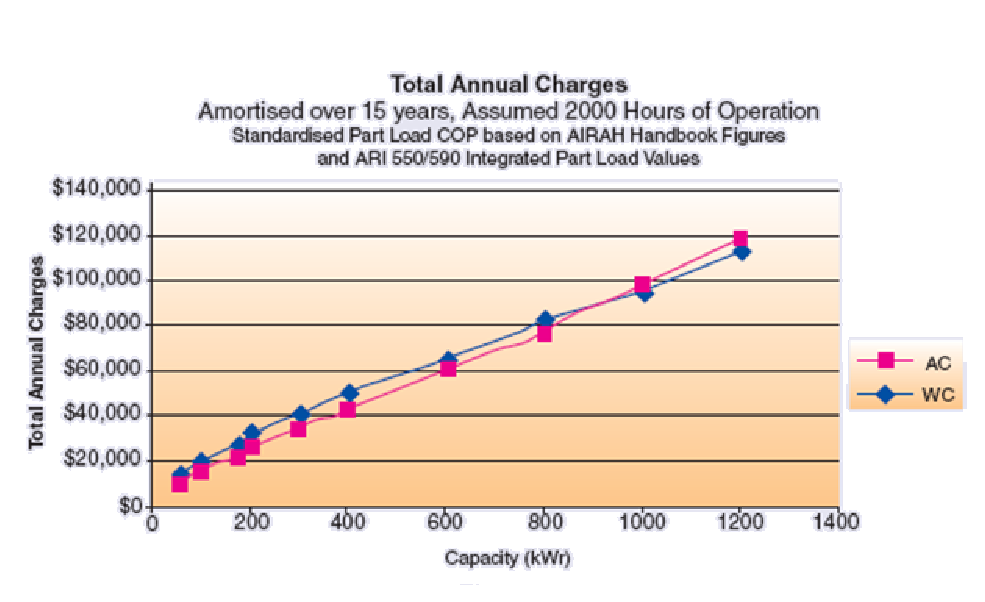
\includegraphics[scale=0.8]{graphics/economic_crossover_annualized}
                    \caption{Economic Cross-over of Annualized Charges Air-cooled to Water-cooled for 2000 Hours of Operations (in US \$)}
                    \label{fig:economic_crossover_annualized}
                \end{figure}
                \begin{figure}[h!tb]
                    \centering
                    \resizebox{\textwidth}{!}{ % Fazendo a tabela caber no espaco da pagina
                    \includegraphics[scale=0.5]{graphics/life_cycle_costs_water_cooled_air_cooled}}
                    \captionof{table}{Life Cycle Costs of Water-cooled and Air-cooled Solutions}
                    \label{tab:life_cycle_costs_water_cooled_air_cooled}
                \end{figure}
                the annual cost for water cooling and air cooling (including charges, maintenance, equipment) do not differ by a large amount as seen in  Table \ref{tab:life_cycle_costs_water_cooled_air_cooled} and Figure \ref{fig:economic_crossover_annualized}. In this way, the main benefit brought by water cooling is the footprint reduction which can increase the server density in a data center.

